\documentclass[9pt,letterpaper]{extarticle}
\usepackage[margin=0.48in,top=0.45in,bottom=0.45in]{geometry}
\usepackage{booktabs}
\usepackage{tabularx}
\usepackage{multirow}
\usepackage{graphicx}
\usepackage{amsmath,amssymb}
\usepackage{xcolor}
\usepackage{enumitem}
\usepackage{caption}
\usepackage{subcaption}
\usepackage{hyperref}
\usepackage{fancyhdr}
\usepackage{microtype}
\usepackage{array}

\definecolor{navy}{HTML}{1F4E78}
\definecolor{slate}{HTML}{2B5C8F}
\definecolor{crimson}{HTML}{842029}
\definecolor{forest}{HTML}{0F5132}
\definecolor{boxbg}{HTML}{F4F7FA}

\hypersetup{
    colorlinks=true,
    linkcolor=navy,
    urlcolor=navy,
    citecolor=navy
}

\captionsetup{font={footnotesize,sf},labelfont={bf,color=navy},skip=3pt}
\setlength{\parindent}{0pt}
\setlength{\parskip}{3pt}
\setlength{\tabcolsep}{3.8pt}
\renewcommand{\arraystretch}{1.06}

\pagestyle{fancy}
\fancyhf{}
\fancyhead[L]{\footnotesize\sffamily\textcolor{navy}{\textbf{Skill Safety Index: Empirical Evaluation Across Stanford TaskNet, O*NET 31.0 Tasks, and O*NET 31.0 Skills}}}
\fancyhead[R]{\footnotesize\sffamily\textcolor{gray}{Results Brief $\cdot$ November 2026}}
\fancyfoot[C]{\footnotesize\sffamily\thepage\ of 4}
\renewcommand{\headrulewidth}{0.4pt}

\begin{document}

% ==============================================================================
% PAGE 1: TITLE, UPFRONT EXECUTIVE SUMMARY BULLETS, RUBRIC & METHODOLOGY
% ==============================================================================
\begin{center}
    {\Large\sffamily\bfseries\textcolor{navy}{Assisted vs.\ Unassisted Skills: Certainty-Weighted Skill Safety Index Across Stanford TaskNet, O*NET 31.0 Tasks, and O*NET 31.0 Skills}}\\[2pt]
    {\footnotesize\sffamily Joshua Martin $\cdot$ Empirical Pipeline \& Psychometric Evaluation Brief $\cdot$ Repository: \href{https://github.com/joshmartingoogle/Skill-Safety}{github.com/joshmartingoogle/Skill-Safety}}
\end{center}
\vspace{-4pt}

\noindent\fcolorbox{navy}{boxbg}{%
\begin{minipage}{\dimexpr\textwidth-2\fboxsep-2\fboxrule\relax}
\vspace{2pt}
{\small\sffamily\bfseries\textcolor{navy}{Executive Summary of Findings (Upfront)}}
\begin{itemize}[leftmargin=1.3em,itemsep=1.2pt,topsep=2pt,parsep=0pt]
    \item \textbf{Directional Standardization \& Certainty-Weighted Pipeline ($N=530$ Items):} We standardized the six-item Skill Safety Index rubric ($N_1$ Fallback, $N_2$ Live Performance, $N_3$ No-AI Rules, $N_4$ Checking, $N_5$ Foundation, and $S$ Stakes) on a unified $0$--$3$ scale where \textbf{higher scores indicate greater skill safety} (lower unassisted need and lower error stakes: $3=\text{Safest / Assist for Good}$, $0=\text{Least Safe / Must Retain Unassisted Ability}$). Passing every item individually to the Gemini Flash API across the latest \textbf{Stanford TaskNet} ($N=202$), \textbf{O*NET 31.0 Tasks} ($N=118$), and \textbf{O*NET 31.0 Skills} ($N=210$) taxonomies yields high epistemic certainty ($\bar{c}=0.903\text{--}0.917$).
    \item \textbf{Bimodal Overall Distributions Across Taxonomies:} Certainty-weighted Skill Safety Index scores ($I_i \in [0,3]$) exhibit a pronounced \textbf{bimodal distribution} in every taxonomy: \textbf{Stanford TaskNet} ($\text{Mean}=1.239$, $\text{SD}=0.896$, $\text{Median}=1.481$, $\text{IQR}=1.811$), \textbf{O*NET 31.0 Tasks} ($\text{Mean}=1.155$, $\text{SD}=0.910$, $\text{Median}=1.209$, $\text{IQR}=1.547$), and \textbf{O*NET 31.0 Skills} ($\text{Mean}=1.323$, $\text{SD}=1.053$, $\text{Median}=1.173$, $\text{IQR}=2.018$). Across taxonomies, $51.0\%\text{--}54.8\%$ of all items fall in the \emph{low-safety regime} ($I_i < 1.5$), while $21.2\%\text{--}34.3\%$ sit in the \emph{high-safety regime} ($I_i \ge 2.0$).
    \item \textbf{Consistent Cross-Industry Ordering \& Within-Occupation Boundary:} Across all three taxonomies, \textbf{Healthcare (Clinical / Emergency Medicine)} exhibits the lowest skill safety (TaskNet $\text{Mean}=0.620$, O*NET Tasks $0.175$, O*NET Skills $0.499$; $73.7\%\text{--}94.1\%$ low-safety), whereas \textbf{Information \& Technology (Software Developers)} exhibits the highest skill safety (TaskNet $\text{Mean}=1.903$, O*NET Tasks $1.813$, O*NET Skills $1.811$), followed by \textbf{Educational Services} ($1.180\text{--}1.513$) and \textbf{Legal \& Professional Services} ($1.160\text{--}1.631$). Crucially, the safety boundary runs \emph{inside} occupations: in Law and Software Engineering, asynchronous drafting and requirements tasks score high on fallback/live safety ($N_1,N_2 \approx 2\text{--}3$) but low on foundation and checking safety ($N_4,N_5 \approx 0\text{--}1$), while $96.9\%\text{--}100.0\%$ trigger the \emph{learner bypass flag} (juniors can obtain usable AI output without working through foundational reasoning).
    \item \textbf{High Internal Consistency ($\alpha > 0.87$) \& Leave-One-Out Diagnostics:} Cronbach's $\alpha$ on certainty-weighted scores is \textbf{$0.8728$} for TaskNet, \textbf{$0.8764$} for O*NET Tasks, and \textbf{$0.9207$} for O*NET Skills (all well above the $0.70$ threshold). Leave-one-out diagnostics reveal that \textbf{Stakes ($S$)} and \textbf{Foundation ($N_5$)} have the lowest item-rest correlations ($r_{\text{rest}}=0.501\text{--}0.597$); omitting $S$ marginally raises $\alpha$ in TaskNet ($\Delta\alpha=+0.0044$ to $0.8772$) and O*NET Skills ($\Delta\alpha=+0.0069$ to $0.9277$) because foundational junior tasks in software and teaching carry low single-error stakes ($S \ge 2$) despite high learning value ($N_5 \le 1$).
    \item \textbf{Spot Verification Audit ($n=45$ Stratified Subsample):} Independent re-scoring of a random subsample ($15$ items per taxonomy) achieves \textbf{$100.0\%$ gate agreement}, \textbf{$95.9\%$ within-$\pm 1$ dimension agreement} ($83.3\%$ exact), and strong index reliability ($r=0.8994$ overall; $r=0.9864$ on TaskNet, $r=0.8707$ on O*NET Tasks, $r=0.8656$ on O*NET Skills).
\end{itemize}
\vspace{1pt}
\end{minipage}%
}

\vspace{2pt}
{\normalsize\sffamily\bfseries\textcolor{navy}{1. Directionally Consistent Skill Safety Rubric \& Certainty-Weighted Index}}

To ensure unidirectional interpretability across all six scored dimensions, each item in the \emph{Rubric and Index} specification is oriented so that a higher score ($0$ to $3$) corresponds to \textbf{greater skill safety}---meaning \textbf{lower unassisted need} ($N_1\text{--}N_5$) and \textbf{lower error stakes} ($S$). First, the model evaluates the \textbf{AI-Assistability Gate} ($g_i \in \{0,1\}$): whether current AI can generate substantive task content (a draft, analysis, plan, or verification check). Second, for each dimension $k \in \{N_1, N_2, N_3, N_4, N_5, S\}$, the pipeline elicits a one-sentence occupation-specific justification, an integer safety score $x_{i,k} \in \{0,1,2,3\}$, and an epistemic certainty score $c_{i,k} \in [0,1]$. Third, the model records the binary \textbf{Learning Flag} ($L_i \in \{0,1\}$: whether a novice using AI in the ordinary way can obtain a usable result without working through the underlying reasoning). The \textbf{Certainty-Weighted Skill Safety Index} $I_i \in [0,3]$ (and normalized score $I_i^{\text{norm}} = I_i/3 \in [0,1]$) is computed as:
\begin{equation*}
I_i = \frac{\sum_{k \in \{N_1, N_2, N_3, N_4, N_5, S\}} c_{i,k} \, x_{i,k}}{\sum_{k \in \{N_1, N_2, N_3, N_4, N_5, S\}} c_{i,k}}, \qquad \text{with Cronbach's } \alpha_{\text{CW}} \text{ evaluated on } \tilde{x}_{i,k} = \frac{6 \, c_{i,k}}{\sum_{j} c_{i,j}} x_{i,k}.
\end{equation*}

\begin{table}[h!]
\centering
\caption{Directionally Standardized Skill Safety Index Rubric ($0 = \text{Lowest Skill Safety}$, $3 = \text{Highest Skill Safety}$)}
\label{tab:rubric}
\scriptsize
\begin{tabularx}{\textwidth}{@{}p{0.38in}p{1.95in}XXXX@{}}
\toprule
\textbf{Item} & \textbf{Dimension \& Core Question} & \textbf{0 (Lowest Safety: Highest Need/Stakes)} & \textbf{1 (Low Safety: High Need/Stakes)} & \textbf{2 (Moderate Safety: Low Need/Stakes)} & \textbf{3 (Highest Safety: Lowest Need/Stakes)} \\
\midrule
\textbf{N1} & \textbf{Fallback:} If AI were unexpectedly unavailable when this came up, how long could it wait? & It cannot wait at all. \emph{(e.g., manual flying on autopilot disconnect)} & A few hours. & Until the next day. & Several days or more. \emph{(e.g., drafting campaign summary)} \\
\addlinespace[1.5pt]
\textbf{N2} & \textbf{Live Performance:} How often done on the spot in front of others with no chance to consult AI? & Daily. \emph{(e.g., answering judge's live question)} & About weekly. & About monthly. & Rarely or never. \emph{(e.g., reconciling accounts)} \\
\addlinespace[1.5pt]
\textbf{N3} & \textbf{No-AI Rules:} How often done where client, employer, court, or privacy rules bar AI? & Daily. \emph{(e.g., client-barred legal matter)} & About weekly. & About monthly. & Rarely or never. \emph{(e.g., internal marketing summary)} \\
\addlinespace[1.5pt]
\textbf{N4} & \textbf{Checking:} To tell whether AI output is right, how much work/reasoning must be repeated? & All of it; work must be redone. \emph{(e.g., legal research memo)} & Much of it; sources or key steps rechecked. & A little; a careful read is enough. & None; a glance or automated test suffices. \\
\addlinespace[1.5pt]
\textbf{N5} & \textbf{Foundation:} Is doing this by hand how people in this occupation build later skills? & Yes; training \& entry-level work built around it. & Mostly; usual way later skill is learned. & Partly; one of several ways learned. & No; nothing later is learned by doing this. \\
\addlinespace[1.5pt]
\textbf{S} & \textbf{Stakes:} If gotten wrong once and uncaught, what is the typical harm/cost? & Serious irreversible or multi-year harm to a person. & Lasting client/org cost (lost money or sanction). & Fixed within weeks; others are delayed. & Fixed within a day; no one outside team affected. \\
\bottomrule
\end{tabularx}
\end{table}

\newpage
% ==============================================================================
% PAGE 2: SUMMARY STATISTICS OVERALL & BY INDUSTRY + OVERALL DENSITY PLOTS
% ==============================================================================
{\normalsize\sffamily\bfseries\textcolor{navy}{2. Summary Statistics Overall and by Industry Across Taxonomies}}

We source the latest versions of all three taxonomies across the six matched benchmark occupations/industries: (1) \textbf{Stanford TaskNet} (Nov 17, 2026 release; $N=202$ worker-interview task statements), (2) \textbf{O*NET 31.0 Tasks} (\texttt{task\_statements.csv}; $N=118$ incumbent/expert task statements), and (3) \textbf{O*NET 31.0 Skills} (\texttt{essential\_skills.csv} + \texttt{transferable\_skills.csv} paired with official activity descriptions from \texttt{content\_model\_reference.csv}; $35 \text{ skills} \times 6 \text{ occupations} = 210$ items). Table~\ref{tab:summary_stats} reports summary statistics overall and by industry, and Figure~\ref{fig:overall_densities} displays the overall density distributions.

\begin{table}[h!]
\centering
\caption{Certainty-Weighted Skill Safety Index ($I_i \in [0,3]$) Summary Statistics Overall and by Industry}
\label{tab:summary_stats}
\scriptsize
\begin{tabularx}{\textwidth}{@{}l r r r r r r r r r r r@{}}
\toprule
\textbf{Taxonomy \& Industry Group} & \textbf{$N$} & \textbf{Gate\%} & \textbf{Mean} & \textbf{SD} & \textbf{Median} & \textbf{IQR} & \textbf{P25--P75} & \textbf{Min--Max} & \textbf{Norm} & \textbf{Cert.} & \textbf{Safe\% / Low\%} \\
\midrule
\multicolumn{12}{@{}l}{\textbf{Panel A: Stanford TaskNet (Latest Release, Nov 2026)}} \\
\textbf{Overall (All Items)} & \textbf{202} & \textbf{78.7\%} & \textbf{1.239} & \textbf{0.896} & \textbf{1.481} & \textbf{1.811} & \textbf{0.20--2.01} & \textbf{0.00--2.85} & \textbf{0.413} & \textbf{0.915} & \textbf{27.7\% / 51.0\%} \\
\quad Overall (AI-Assistable Gate = True) & 159 & 100.0\% & 1.444 & 0.846 & 1.670 & 1.312 & 0.72--2.03 & 0.00--2.85 & 0.481 & 0.906 & 34.0\% / 39.0\% \\
\quad Healthcare: Clinical Medicine (EM Physicians) & 38 & 81.6\% & 0.620 & 0.901 & 0.000 & 1.538 & 0.00--1.54 & 0.00--2.52 & 0.207 & 0.948 & 13.2\% / 73.7\% \\
\quad Hospitality \& Food Services (Dishwashers) & 13 & 0.0\% & 0.753 & 0.723 & 0.625 & 0.199 & 0.47--0.67 & 0.00--2.85 & 0.251 & 0.944 & 7.7\% / 92.3\% \\
\quad Healthcare: Personal Care (Care Aides) & 36 & 55.6\% & 0.773 & 0.890 & 0.306 & 1.372 & 0.00--1.37 & 0.00--2.66 & 0.258 & 0.917 & 19.4\% / 77.8\% \\
\quad Legal \& Professional Services (Lawyers) & 32 & 96.9\% & 1.451 & 0.520 & 1.633 & 0.561 & 1.15--1.71 & 0.15--2.52 & 0.484 & 0.909 & 9.4\% / 43.8\% \\
\quad Educational Services (Elem.\ Teachers) & 39 & 84.6\% & 1.513 & 0.944 & 1.830 & 1.865 & 0.47--2.34 & 0.00--2.85 & 0.504 & 0.903 & 46.2\% / 41.0\% \\
\quad Information \& Technology (Software Devs) & 44 & 100.0\% & 1.903 & 0.370 & 1.995 & 0.483 & 1.68--2.16 & 0.96--2.52 & 0.634 & 0.892 & 50.0\% / 11.4\% \\
\midrule
\multicolumn{12}{@{}l}{\textbf{Panel B: O*NET 31.0 Tasks (\texttt{task\_statements.csv})}} \\
\textbf{Overall (All Items)} & \textbf{118} & \textbf{79.7\%} & \textbf{1.155} & \textbf{0.910} & \textbf{1.209} & \textbf{1.547} & \textbf{0.30--1.85} & \textbf{0.00--3.00} & \textbf{0.385} & \textbf{0.917} & \textbf{21.2\% / 54.2\%} \\
\quad Overall (AI-Assistable Gate = True) & 94 & 100.0\% & 1.291 & 0.893 & 1.641 & 1.643 & 0.32--1.97 & 0.00--2.84 & 0.430 & 0.910 & 25.5\% / 46.8\% \\
\quad Healthcare: Clinical Medicine (EM Physicians) & 17 & 82.4\% & 0.175 & 0.530 & 0.000 & 0.000 & 0.00--0.00 & 0.00--2.18 & 0.058 & 0.960 & 5.9\% / 94.1\% \\
\quad Hospitality \& Food Services (Dishwashers) & 13 & 0.0\% & 0.958 & 0.836 & 0.782 & 1.104 & 0.32--1.43 & 0.00--3.00 & 0.319 & 0.931 & 7.7\% / 76.9\% \\
\quad Legal \& Professional Services (Lawyers) & 22 & 100.0\% & 1.160 & 0.697 & 1.461 & 0.990 & 0.66--1.66 & 0.00--2.18 & 0.387 & 0.917 & 9.1\% / 54.5\% \\
\quad Educational Services (Elem.\ Teachers) & 38 & 89.5\% & 1.309 & 0.953 & 1.574 & 1.862 & 0.32--2.18 & 0.00--2.84 & 0.436 & 0.908 & 28.9\% / 47.4\% \\
\quad Healthcare: Personal Care (Care Aides) & 11 & 63.6\% & 1.342 & 1.104 & 1.683 & 1.860 & 0.15--2.01 & 0.00--2.83 & 0.447 & 0.906 & 27.3\% / 45.5\% \\
\quad Information \& Technology (Software Devs) & 17 & 100.0\% & 1.813 & 0.400 & 1.817 & 0.536 & 1.65--2.18 & 1.15--2.35 & 0.604 & 0.888 & 41.2\% / 17.6\% \\
\midrule
\multicolumn{12}{@{}l}{\textbf{Panel C: O*NET 31.0 Skills (\texttt{essential\_skills.csv} + \texttt{transferable\_skills.csv})}} \\
\textbf{Overall (All Items)} & \textbf{210} & \textbf{81.9\%} & \textbf{1.323} & \textbf{1.053} & \textbf{1.173} & \textbf{2.018} & \textbf{0.32--2.34} & \textbf{0.00--3.00} & \textbf{0.441} & \textbf{0.903} & \textbf{34.3\% / 54.8\%} \\
\quad Overall (AI-Assistable Gate = True) & 172 & 100.0\% & 1.446 & 1.016 & 1.643 & 1.877 & 0.48--2.35 & 0.00--3.00 & 0.482 & 0.899 & 38.4\% / 48.8\% \\
\quad Healthcare: Clinical Medicine (EM Physicians) & 35 & 82.9\% & 0.499 & 0.844 & 0.000 & 0.547 & 0.00--0.55 & 0.00--2.70 & 0.166 & 0.934 & 11.4\% / 82.9\% \\
\quad Healthcare: Personal Care (Care Aides) & 35 & 77.1\% & 1.060 & 1.026 & 0.641 & 1.850 & 0.15--2.00 & 0.00--3.00 & 0.353 & 0.886 & 25.7\% / 65.7\% \\
\quad Educational Services (Elem.\ Teachers) & 35 & 80.0\% & 1.180 & 1.088 & 0.486 & 1.951 & 0.39--2.34 & 0.00--3.00 & 0.393 & 0.907 & 34.3\% / 65.7\% \\
\quad Legal \& Professional Services (Lawyers) & 35 & 97.1\% & 1.631 & 1.008 & 2.009 & 1.735 & 0.62--2.36 & 0.16--3.00 & 0.544 & 0.901 & 51.4\% / 45.7\% \\
\quad Hospitality \& Food Services (Dishwashers) & 35 & 54.3\% & 1.757 & 1.109 & 2.181 & 2.363 & 0.48--2.84 & 0.16--3.00 & 0.586 & 0.907 & 51.4\% / 42.9\% \\
\quad Information \& Technology (Software Devs) & 35 & 100.0\% & 1.811 & 0.548 & 1.840 & 0.699 & 1.56--2.26 & 0.31--2.69 & 0.604 & 0.886 & 31.4\% / 25.7\% \\
\bottomrule
\multicolumn{12}{@{}p{\textwidth}@{}}{\tiny \emph{Notes:} Gate\% = share of items passing the AI-assistable gate ($g_i=1$). Norm = normalized index $I_i/3 \in [0,1]$. Cert.\ = mean assessment certainty $\bar{c}_i \in [0,1]$. Safe\% = share of items with $I_i \ge 2.0$ (high safety / assist for good); Low\% = share of items with $I_i < 1.5$ (low safety / high unassisted need or stakes).}
\end{tabularx}
\end{table}

\vspace{-4pt}
\begin{figure}[h!]
\centering
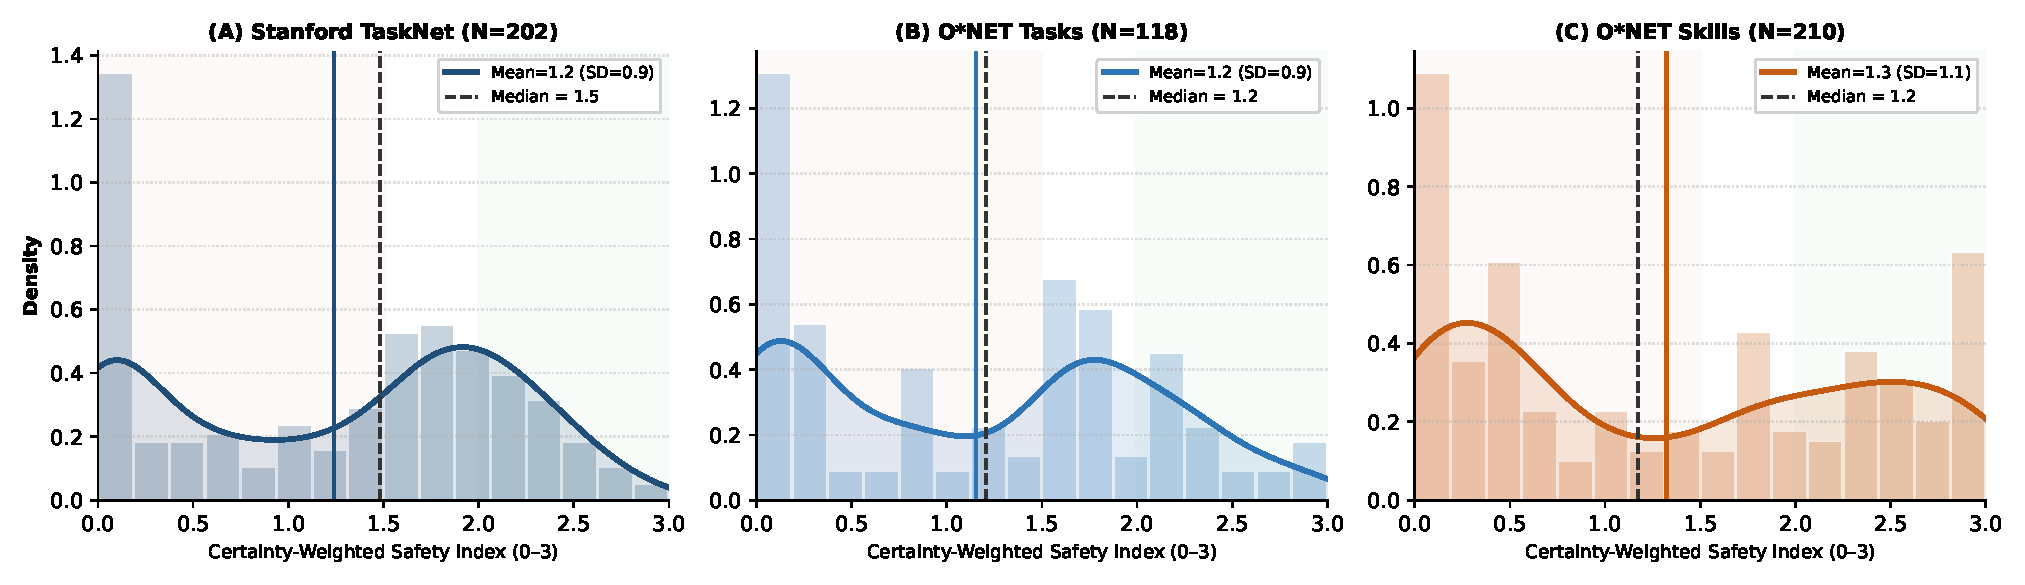
\includegraphics[width=0.99\textwidth]{figures/density_overall_all_taxonomies.pdf}\\[-2pt]
\begin{subfigure}[b]{0.325\textwidth}
    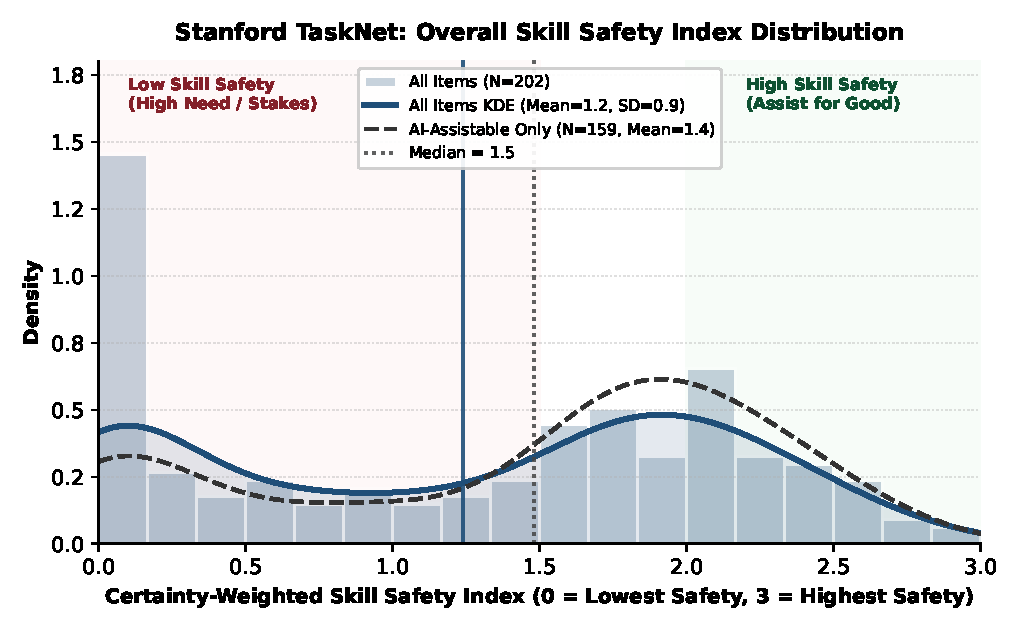
\includegraphics[width=\textwidth]{figures/density_overall_tasknet.pdf}
\end{subfigure}\hfill
\begin{subfigure}[b]{0.325\textwidth}
    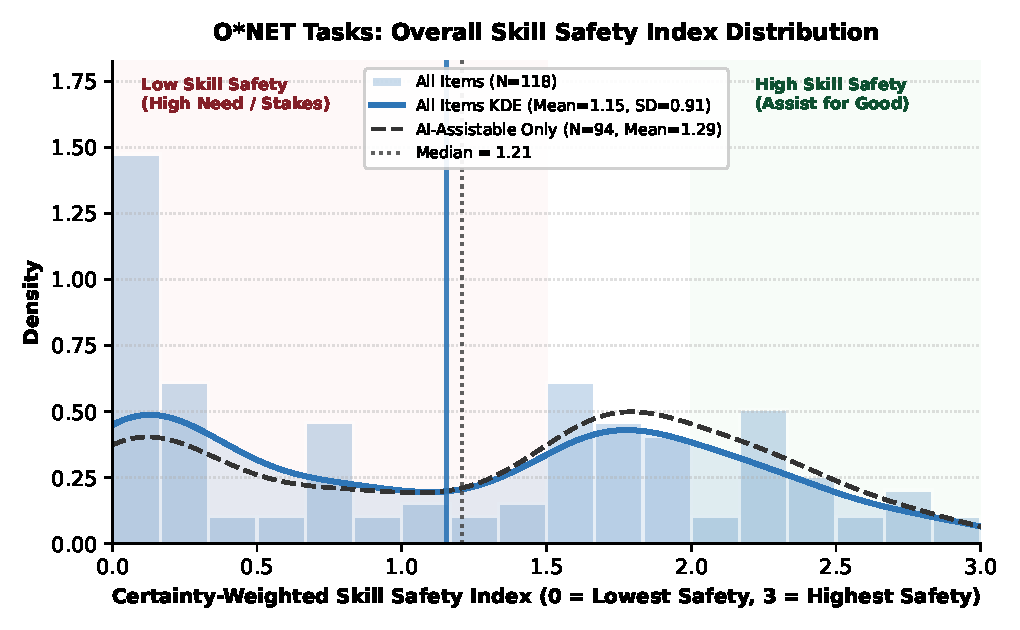
\includegraphics[width=\textwidth]{figures/density_overall_onet_tasks.pdf}
\end{subfigure}\hfill
\begin{subfigure}[b]{0.325\textwidth}
    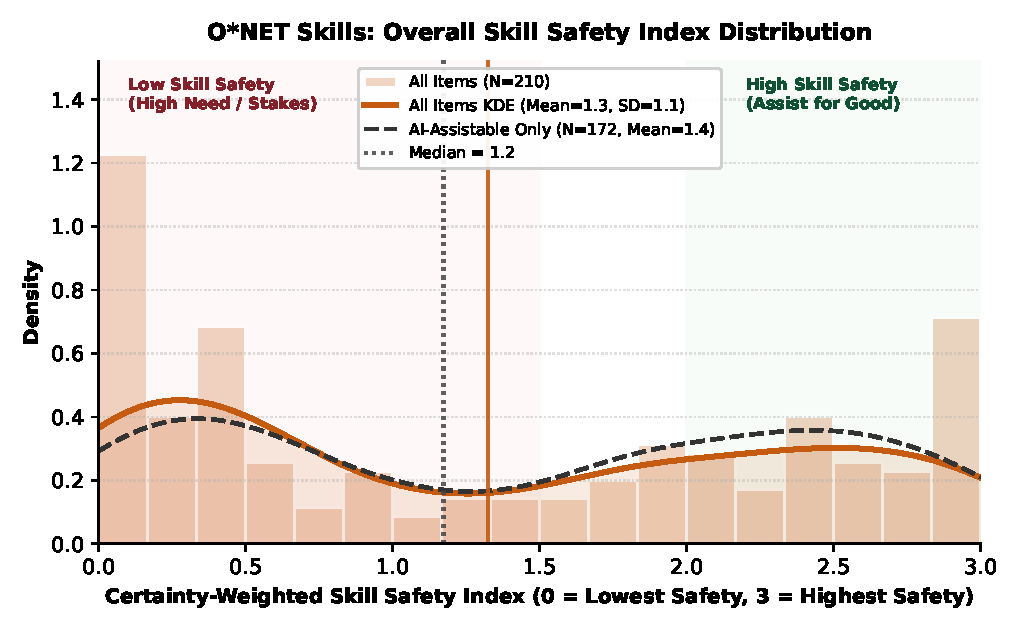
\includegraphics[width=\textwidth]{figures/density_overall_onet_skills.pdf}
\end{subfigure}
\caption{Overall Density Distributions of Certainty-Weighted Skill Safety Index Scores Across Taxonomies (Top: Side-by-Side Comparison; Bottom: Individual Taxonomy Distributions Comparing All Items vs.\ AI-Assistable Gated Items)}
\label{fig:overall_densities}
\end{figure}

\newpage
% ==============================================================================
% PAGE 3: PANELED DENSITY PLOTS BY INDUSTRY FOR ALL THREE TAXONOMIES
% ==============================================================================
{\normalsize\sffamily\bfseries\textcolor{navy}{3. Paneled Density Distributions by Industry Across All Three Taxonomies}}

Figure~\ref{fig:industry_panels} presents the 6-industry paneled kernel density and histogram distributions for \textbf{Stanford TaskNet} (Panel A), \textbf{O*NET 31.0 Tasks} (Panel B), and \textbf{O*NET 31.0 Skills} (Panel C). Across all three taxonomies, acute clinical healthcare tasks cluster near zero safety ($I_i \approx 0$), software development clusters in the moderate-to-high safety regime ($I_i \approx 1.8\text{--}2.2$), and education and legal services span both regimes, demonstrating that the boundary between safe permanent assistance and essential unassisted human capability runs \emph{within} occupations and industries.

\begin{figure}[ht!]
\centering
\begin{subfigure}[b]{0.96\textwidth}
    \centering
    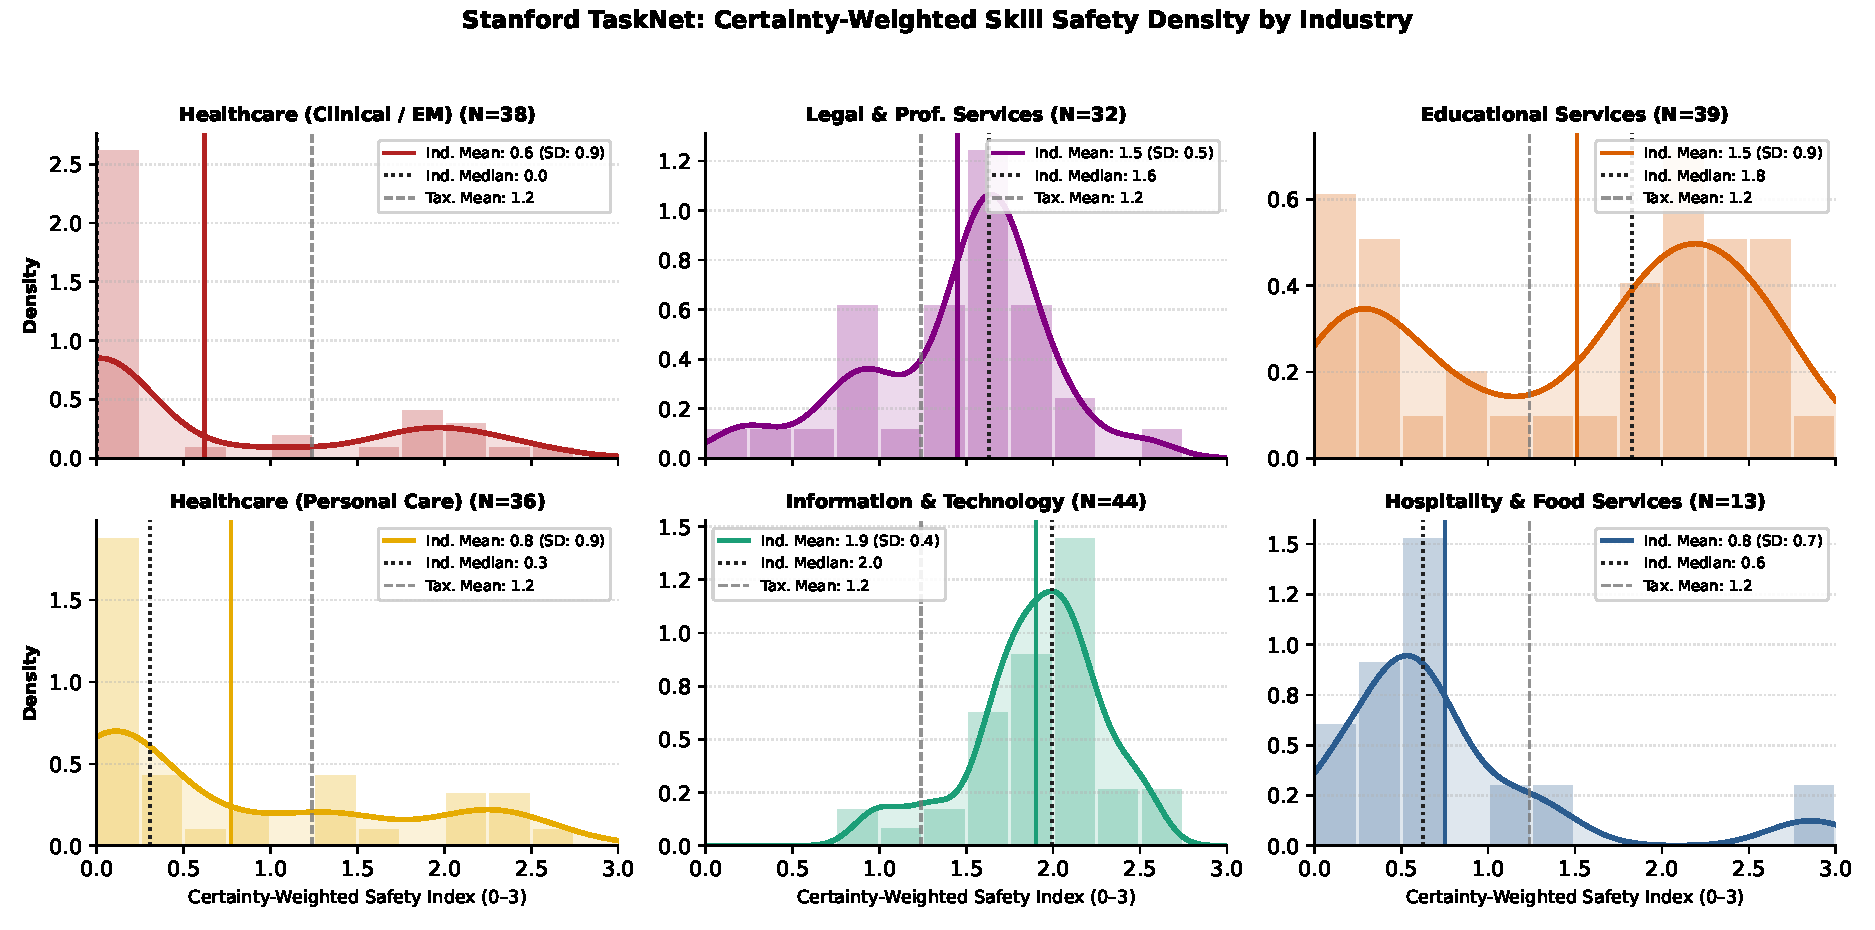
\includegraphics[width=\textwidth,height=0.242\textheight,keepaspectratio]{figures/density_by_industry_tasknet.pdf}
    \caption{Stanford TaskNet ($N=202$): Paneled Skill Safety Density Distribution by Industry}
\end{subfigure}\\[1pt]
\begin{subfigure}[b]{0.96\textwidth}
    \centering
    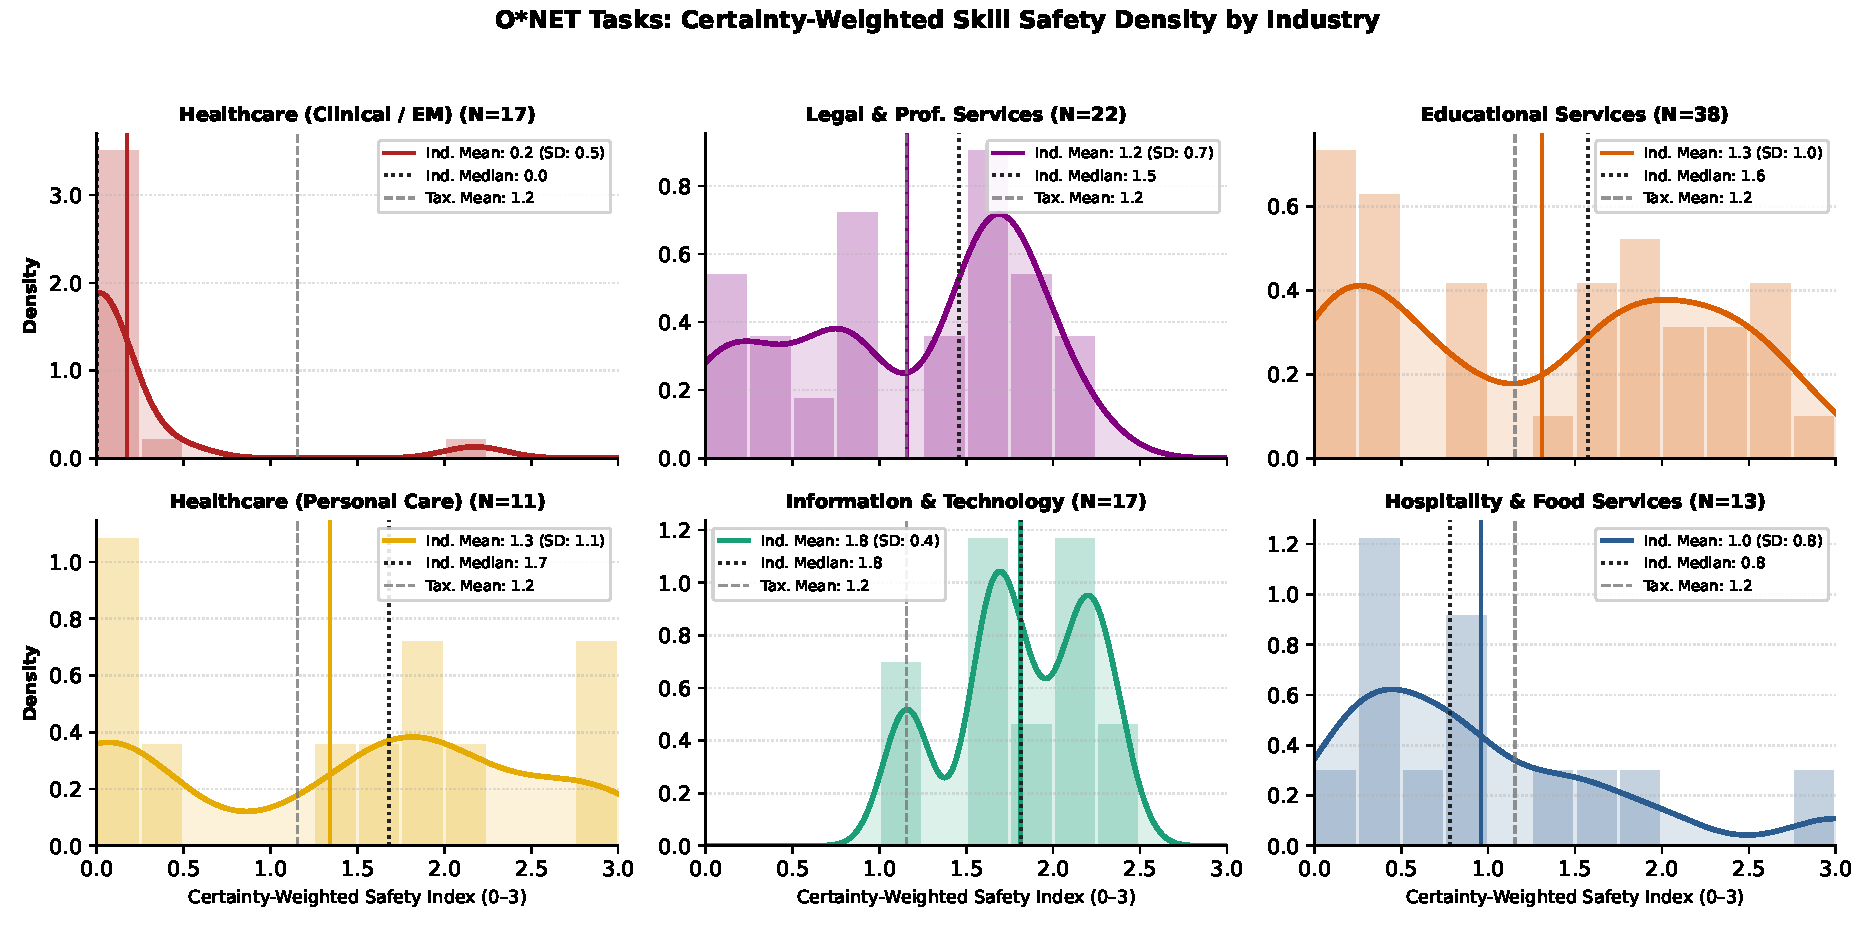
\includegraphics[width=\textwidth,height=0.242\textheight,keepaspectratio]{figures/density_by_industry_onet_tasks.pdf}
    \caption{O*NET 31.0 Tasks ($N=118$): Paneled Skill Safety Density Distribution by Industry}
\end{subfigure}\\[1pt]
\begin{subfigure}[b]{0.96\textwidth}
    \centering
    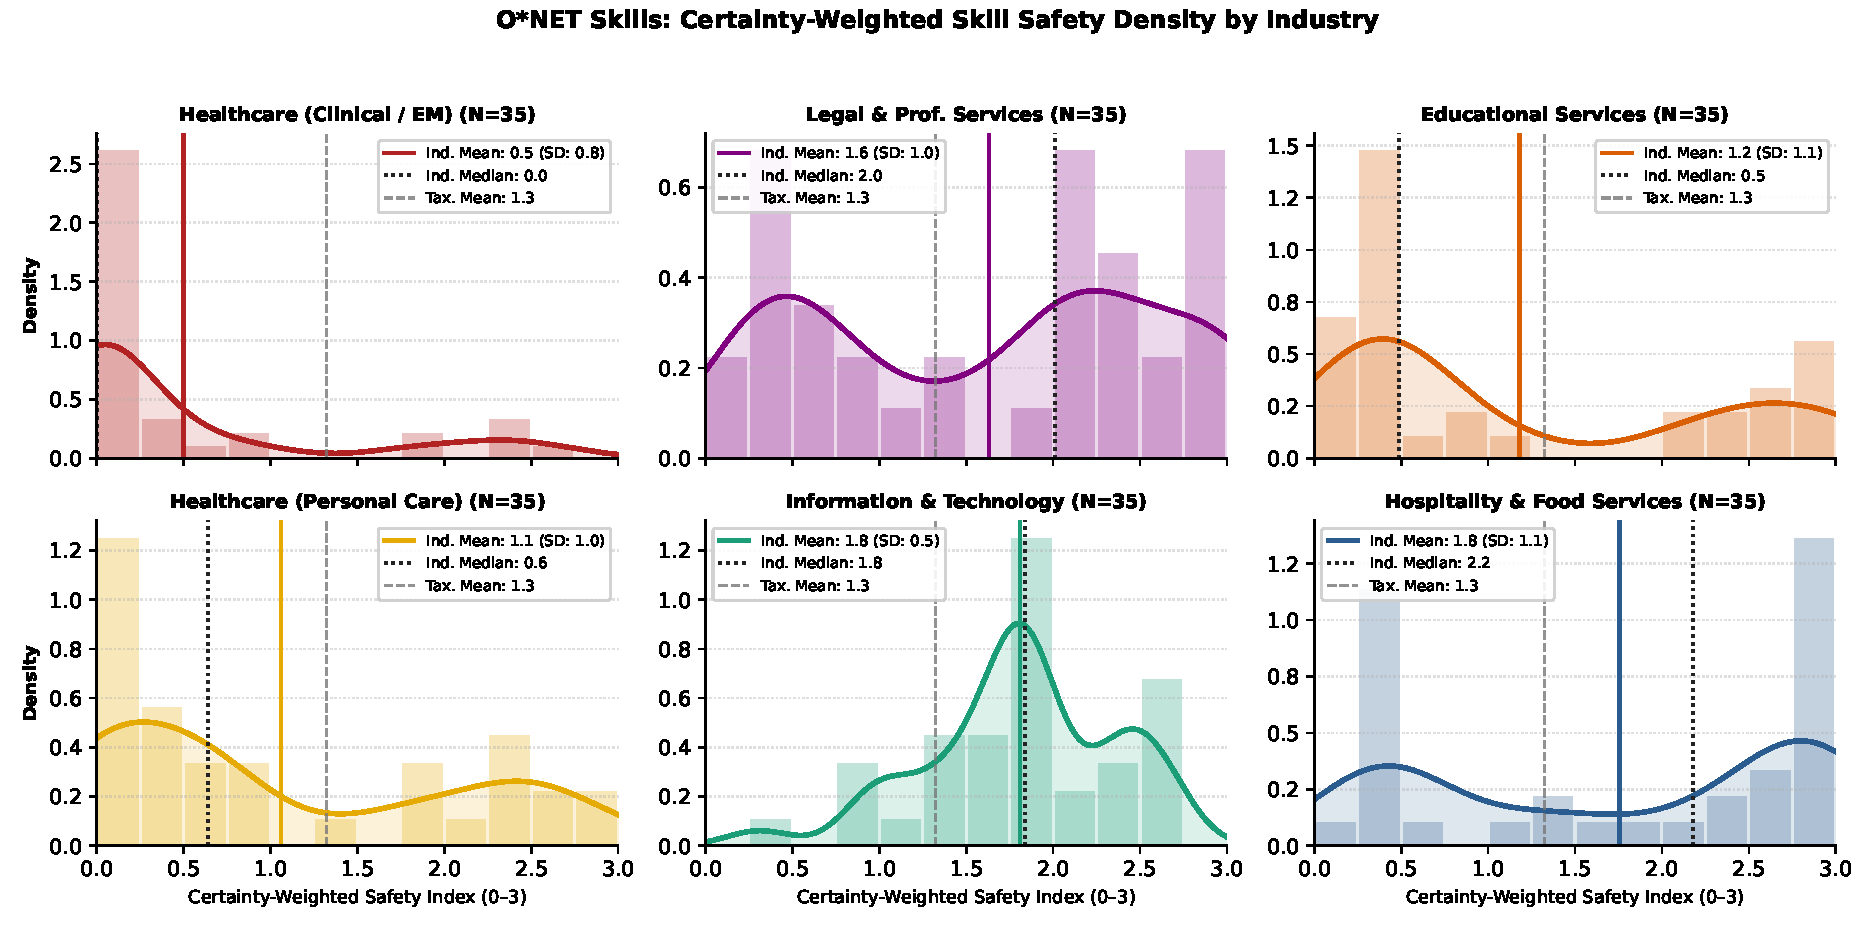
\includegraphics[width=\textwidth,height=0.242\textheight,keepaspectratio]{figures/density_by_industry_onet_skills.pdf}
    \caption{O*NET 31.0 Skills ($N=210$): Paneled Skill Safety Density Distribution by Industry}
\end{subfigure}
\caption{Paneled Kernel Density and Histogram Distributions of Certainty-Weighted Skill Safety Index Scores by Industry}
\label{fig:industry_panels}
\end{figure}

\newpage
% ==============================================================================
% PAGE 4: CRONBACH ALPHA & LEAVE-ONE-OUT DIAGNOSTICS + SPOT VERIFICATION
% ==============================================================================
{\normalsize\sffamily\bfseries\textcolor{navy}{4. Scale Reliability (Cronbach's $\alpha$) \& Leave-One-Out Item Diagnostics}}

Table~\ref{tab:cronbach} reports Cronbach's $\alpha$ on both certainty-weighted item contributions ($\alpha_{\text{CW}}$) and unweighted scores ($\alpha_{\text{Raw}}$), together with complete \textbf{leave-one-out ($\alpha_{\text{if item deleted}}$)} diagnostics and item-rest correlations ($r_{\text{rest}}$). While scale reliability exceeds the $0.70$ benchmark in every taxonomy ($\alpha_{\text{CW}} = 0.8728$ in TaskNet, $0.8764$ in O*NET Tasks, and $0.9207$ in O*NET Skills), performing the full leave-one-out analysis across all three taxonomies reveals an important structural property of the rubric:
\begin{itemize}[leftmargin=1.3em,itemsep=1pt,topsep=1pt]
    \item \textbf{Core Operational Need ($N_1\text{--}N_4$) Drives Scale Cohesion:} Fallback ($N_1$), Live Performance ($N_2$), No-AI Rules ($N_3$), and Checking ($N_4$) exhibit strong item-rest correlations ($r_{\text{rest}} = 0.730\text{--}0.860$). Removing any of $N_1\text{--}N_4$ substantially reduces $\alpha_{\text{CW}}$ by $-0.0113$ to $-0.0519$.
    \item \textbf{Orthogonality of Stakes ($S$) and Foundation ($N_5$):} Stakes ($S$) has the lowest item-rest correlation across all three taxonomies ($r_{\text{rest}} = 0.501$ in TaskNet, $0.559$ in O*NET Tasks, $0.597$ in O*NET Skills), followed by Foundation ($N_5$, $r_{\text{rest}} = 0.543\text{--}0.807$). Deleting $S$ slightly increases $\alpha_{\text{CW}}$ in Stanford TaskNet ($\Delta\alpha = +0.0044$, from $0.8728$ to $0.8772$) and O*NET Skills ($\Delta\alpha = +0.0069$, from $0.9207$ to $0.9277$). Substantively, this confirms Hypothesis H1/H2: many entry-level skill-building tasks in software engineering and teaching have high foundational importance ($N_5 \in \{0,1\}$) but low single-error stakes ($S \in \{2,3\}$) because automated tests or supervisory review catch errors before external harm occurs.
\end{itemize}

\begin{table}[h!]
\centering
\caption{Cronbach's $\alpha$ and Leave-One-Out ($\alpha_{\text{if item deleted}}$) Diagnostics Across Taxonomies}
\label{tab:cronbach}
\scriptsize
\begin{tabularx}{\textwidth}{@{}l r r r r r | r r r r r | r r r r r@{}}
\toprule
& \multicolumn{5}{c|}{\textbf{Stanford TaskNet ($N=202$)}} & \multicolumn{5}{c|}{\textbf{O*NET 31.0 Tasks ($N=118$)}} & \multicolumn{5}{c}{\textbf{O*NET 31.0 Skills ($N=210$)}} \\
& \multicolumn{5}{c|}{$\alpha_{\text{CW}} = \mathbf{0.8728}$ \quad ($\alpha_{\text{Raw}} = 0.8718$)} & \multicolumn{5}{c|}{$\alpha_{\text{CW}} = \mathbf{0.8764}$ \quad ($\alpha_{\text{Raw}} = 0.8747$)} & \multicolumn{5}{c}{$\alpha_{\text{CW}} = \mathbf{0.9207}$ \quad ($\alpha_{\text{Raw}} = 0.9202$)} \\
\cmidrule(lr){2-6} \cmidrule(lr){7-11} \cmidrule(l){12-16}
\textbf{Rubric Item} & \textbf{Mean} & \textbf{Cert} & \textbf{$r_{\text{rest}}$} & \textbf{$\alpha_{-k}$} & \textbf{$\Delta\alpha$} & \textbf{Mean} & \textbf{Cert} & \textbf{$r_{\text{rest}}$} & \textbf{$\alpha_{-k}$} & \textbf{$\Delta\alpha$} & \textbf{Mean} & \textbf{Cert} & \textbf{$r_{\text{rest}}$} & \textbf{$\alpha_{-k}$} & \textbf{$\Delta\alpha$} \\
\midrule
\textbf{N1: Fallback} & 1.830 & 0.928 & 0.782 & 0.8321 & $-0.0407$ & 1.687 & 0.925 & 0.749 & 0.8453 & $-0.0311$ & 1.556 & 0.912 & 0.807 & 0.9027 & $-0.0180$ \\
\textbf{N2: Live Perf.} & 1.675 & 0.952 & 0.776 & 0.8377 & $-0.0351$ & 1.266 & 0.949 & 0.731 & 0.8512 & $-0.0253$ & 1.389 & 0.942 & 0.851 & 0.8971 & $-0.0236$ \\
\textbf{N3: No-AI Rules} & 1.357 & 0.882 & 0.833 & 0.8209 & $-0.0519$ & 1.276 & 0.883 & 0.825 & 0.8285 & $-0.0479$ & 1.611 & 0.879 & 0.860 & 0.8938 & $-0.0269$ \\
\textbf{N4: Checking} & 0.923 & 0.901 & 0.730 & 0.8505 & $-0.0223$ & 0.924 & 0.901 & 0.739 & 0.8532 & $-0.0232$ & 1.057 & 0.880 & 0.799 & 0.9094 & $-0.0113$ \\
\textbf{N5: Foundation} & 0.662 & 0.897 & 0.543 & 0.8726 & $-0.0002$ & 0.671 & 0.908 & 0.596 & 0.8710 & $-0.0054$ & 1.120 & 0.901 & 0.807 & 0.9018 & $-0.0189$ \\
\textbf{S: Stakes} & 0.988 & 0.931 & 0.501 & \textbf{0.8772} & $\mathbf{+0.0044}$ & 1.105 & 0.933 & 0.559 & 0.8741 & $-0.0023$ & 1.205 & 0.908 & 0.597 & \textbf{0.9277} & $\mathbf{+0.0069}$ \\
\bottomrule
\end{tabularx}
\end{table}

\vspace{-2pt}
{\normalsize\sffamily\bfseries\textcolor{navy}{5. Spot Verification on Stratified Random Subsample ($n=45$ Items)}}

To verify scoring stability and audit item-level reasoning, we drew a stratified random subsample of $n=45$ items ($15$ per taxonomy) and conducted an independent second scoring pass. Table~\ref{tab:spot_summary} summarizes test--retest agreement metrics by taxonomy and illustrates representative verified items across industries. Across all $45$ verified items, AI-assistability gate agreement is \textbf{$100.0\%$}, within-$\pm 1$ dimension agreement is \textbf{$95.9\%$} ($83.3\%$ exact), and certainty-weighted index correlation is \textbf{$r=0.8994$} ($\text{MAE}=0.2025$). Agreement is highest on concrete Stanford TaskNet statements ($r=0.9864$, $\text{MAE}=0.0708$, $88.9\%$ exact, $100.0\%$ within $\pm 1$) and slightly lower on broader O*NET Tasks ($r=0.8707$) and abstract O*NET Skills ($r=0.8656$), particularly on $N_3$ (No-AI Rules, $66.7\%\text{--}73.3\%$ exact) where employer policies vary.

\begin{table}[h!]
\centering
\caption{Spot Verification Audit: Pass-to-Pass Agreement ($n=45$) and Representative Verified Subsample Items}
\label{tab:spot_summary}
\scriptsize
\begin{tabularx}{\textwidth}{@{}l r r r r r r r r r r r@{}}
\toprule
\textbf{Subsample Group} & \textbf{$n$} & \textbf{Index $r$} & \textbf{MAE} & \textbf{Gate\%} & \textbf{Exact\%} & \textbf{$\pm 1$ Agree\%} & \textbf{N1\%} & \textbf{N2\%} & \textbf{N3\%} & \textbf{N4\%} & \textbf{N5\% / S\%} \\
\midrule
\textbf{All Verified Items} & \textbf{45} & \textbf{0.8994} & \textbf{0.2025} & \textbf{100.0\%} & \textbf{83.3\%} & \textbf{95.9\%} & \textbf{88.9\%} & \textbf{86.7\%} & \textbf{75.6\%} & \textbf{84.4\%} & \textbf{84.4\% / 80.0\%} \\
Stanford TaskNet Subsample & 15 & 0.9864 & 0.0708 & 100.0\% & 88.9\% & 100.0\% & 86.7\% & 86.7\% & 86.7\% & 86.7\% & 86.7\% / 100.0\% \\
O*NET 31.0 Tasks Subsample & 15 & 0.8707 & 0.2478 & 100.0\% & 78.9\% & 95.6\% & 93.3\% & 80.0\% & 66.7\% & 86.7\% & 86.7\% / 60.0\% \\
O*NET 31.0 Skills Subsample & 15 & 0.8656 & 0.2890 & 100.0\% & 82.2\% & 92.2\% & 86.7\% & 93.3\% & 73.3\% & 80.0\% & 80.0\% / 80.0\% \\
\bottomrule
\end{tabularx}

\vspace{3pt}
\begin{tabularx}{\textwidth}{@{}p{0.82in}p{0.92in}X r r r c c@{}}
\toprule
\textbf{Taxonomy (ID)} & \textbf{Industry (Occ.)} & \textbf{Sampled Task / Skill Statement} & \textbf{Pass 1} & \textbf{Pass 2} & \textbf{Cert.} & \textbf{$[N_1..N_5,S]_1$} & \textbf{$[N_1..N_5,S]_2$} \\
\midrule
TaskNet (\texttt{S-SWD-07}) & Info.\ \& Tech.\ (Software Devs) & Decompose approved features and product requirements into technical implementation tasks for development teams. & 2.19 & 2.19 & 0.86 & \texttt{[3,2,3,2,1,2]} & \texttt{[3,3,3,1,1,2]} \\
TaskNet (\texttt{S-LAW-16}) & Legal Services (Lawyers) & Check legal citations against source documents and review executed court-required forms for accuracy. & 1.83 & 1.84 & 0.91 & \texttt{[3,3,3,1,0,1]} & \texttt{[2,3,3,1,1,1]} \\
TaskNet (\texttt{S-LAW-08}) & Legal Services (Lawyers) & Draft and file motions, briefs, pleadings, complaints, and related court filings for active cases. & 1.66 & 1.81 & 0.95 & \texttt{[3,3,2,1,0,1]} & \texttt{[3,3,3,1,0,1]} \\
O*NET Task (\texttt{6557}) & Education (Elem.\ Teachers) & Prepare for assigned classes and show written evidence of preparation upon request of immediate supervisors. & 2.20 & 2.19 & 0.89 & \texttt{[2,3,3,2,1,2]} & \texttt{[2,3,3,2,1,2]} \\
O*NET Task (\texttt{22722}) & Healthcare: EM (Physicians) & Discuss patients' treatment plans with physicians and other medical professionals. & 0.00 & 0.00 & 0.97 & \texttt{[0,0,0,0,0,0]} & \texttt{[0,0,0,0,0,0]} \\
O*NET Task (\texttt{11194}) & Hospitality (Dishwashers) & Set up banquet tables. \emph{(Gate = False: hands-on physical setup, low error stakes $S=3$)} & 0.66 & 0.67 & 0.93 & \texttt{[0,0,0,0,1,3]} & \texttt{[0,0,0,0,1,3]} \\
O*NET Skill (\texttt{2.A.1.e}) & Healthcare: EM (Physicians) & Mathematics: Using mathematics to solve problems (e.g., acute medication dosing calculations in EM). & 0.14 & 0.14 & 0.93 & \texttt{[0,0,1,0,0,0]} & \texttt{[0,0,1,0,0,0]} \\
O*NET Skill (\texttt{2.B.5.a}) & Healthcare: EM (Physicians) & Time Management: Managing one's own time and the time of others in emergency triage. & 0.00 & 0.00 & 0.97 & \texttt{[0,0,0,0,0,0]} & \texttt{[0,0,0,0,0,0]} \\
\bottomrule
\end{tabularx}
\end{table}

\end{document}
